\chapter{Syntax-driven design of neural-specific enhancers in vivo}
\label{chap:chapter 2}

%%%%%%%%%%%%%%%%%%%%%%%%%%%%%%%%%%%%%%%%%%%%%%%%%%%%%%%%%%%%%%%%%%%%%%%%%%%%%%%%
\section{Abstract}
%%%%%%%%%%%%%%%%%%%%%%%%%%%%%%%%%%%%%%%%%%%%%%%%%%%%%%%%%%%%%%%%%%%%%%%%%%%%%%%%

The syntax (order, orientation, and spacing) of transcription factor binding sites (TFBSs) is a key determinant of enhancer activity and specificity. To isolate the contribution of syntax, we constructed a large synthetic MPRA library in which all sequences share the same five TFBSs but vary in their arrangement. Only a fraction of these syntax variants are active, demonstrating the importance of syntax in driving enhancer function. We trained deep learning models to predict enhancer activity from these data and found that enhancer function is readily predictable from syntax alone. Model interpretation revealed that predictions are largely driven by an additive combination of learned 2-site and 3-site configurations, which capture TFBS arrangements significantly associated with function. Guided by the syntax model, we designed 192 synthetic enhancers by either activating an inert sequence or repressing an enhancer that drives ectopic expression patterns. 93\% (179/192) of our designs tuned activity in the intended direction, and 46\% (89/192) exhibited tissue-specific activity. Our results demonstrate that syntax-based modeling provides a powerful and interpretable framework for understanding and engineering enhancer function.

%%%%%%%%%%%%%%%%%%%%%%%%%%%%%%%%%%%%%%%%%%%%%%%%%%%%%%%%%%%%%%%%%%%%%%%%%%%%%%%%
\section{Main}
%%%%%%%%%%%%%%%%%%%%%%%%%%%%%%%%%%%%%%%%%%%%%%%%%%%%%%%%%%%%%%%%%%%%%%%%%%%%%%%%

Enhancers are DNA sequences that control when and where genes are expressed. They function as genetic switches that activate transcription of nearby genes when bound by transcription factor (TF) proteins, often in specific developmental stages or cell types \cite{Levine2010-ry}. Short sequence motifs called transcription factor binding sites (TFBS) drive enhancer activity \cite{Stormo2010-xm}, and many enhancers obey certain organizational rules for these TFBSs that go beyond their mere presence, often referred to as an enhancer’s “grammar” \cite{Jindal2021-zk}. In this view, an enhancer’s function is not only controlled by the number, type, and affinity of the TFBSs it contains (the composition), but also by the relative order, orientation, and spacing of these sites (the syntax). Much like words in a sentence must be ordered correctly to convey meaning, the arrangement of TFBS can affect whether TFs cooperate or interfere, as TF proteins and DNA may have specific interaction requirements.

The specificity of many enhancers makes them attractive tools for use in gene therapy applications that require delivery of a gene to specific tissues or cell types. This has driven significant interest in the computational design of synthetic enhancers with tissue-specific regulatory activity. Many approaches leverage training of deep learning models to predict functional readouts from DNA sequence on large-scale genomic datasets, such as genome-wide chromatin accessibility profiles \cite{Taskiran2023-xz,De_Almeida2023-xu} or massively parallel reporter assays (MPRAs) that measure enhancer activity \cite{De_Almeida2022-aa,Gosai2023-cw,De_Boer2020-mw,White2016-ks}. Once trained, these models can iteratively evaluate and optimize candidate sequences toward a predefined objective, such as maximizing activity in a specific cell type \cite{Gosai2023-cw,Taskiran2023-xz}. More recently, generative modeling has been used to design synthetic enhancers, sampling sequences predicted to drive strong, context-specific gene expression \cite{noauthor_undated-wu,Penzar2023-vr}.

Despite the success of these models, the extent to which they are capable of learning more  complex enhancer grammars remains unclear. Interpretable machine learning methods \cite{Novakovsky2022-ft} have been used to show that models effectively identify binding sites for key transcription factors (TFs) required for tissue-specific activity and recognize common TFBS cooperativity patterns\cite{Avsec2021-sw,De_Almeida2022-aa,Gosai2023-cw,Taskiran2023-xz}. This information has been sufficient to predict enhancer activity in these contexts, but these models have yet to be sufficiently tested on enhancers that exhibit stronger syntax dependencies, where even small changes in motif order, spacing, or orientation can lead to drastic shifts in gene expression, including loss of specificity \cite{Lim2024-ph,Jindal2022-qf,Farley2016-eh}. 

Many of these models are constrained by the relatively small number of higher-order TFBS combinations present in naturally occurring genomic sequences \cite{De_Boer2024-ic}. In contrast, MPRAs performed on synthetically designed sequences enable systematic interrogation of enhancer function with more control over TFBS composition and syntax. These assays break down enhancer complexity into targeted, testable components that are effective for isolating grammatical rules and revealing dependencies that may be difficult to infer from natural sequences \cite{Fromel2024-ux,King2020-hk}.
Here, we present a systematic approach for learning the relationship between DNA sequence and function by combining deep experimental profiling of TFBS syntax with deep learning. 

We first define the necessary and sufficient TFBSs within an enhancer of interest that are used to construct a DNA sequence library where these TFBSs are systematically rearranged. 
We then characterize the regulatory activity of the library in vivo using MPRA and train a neural network to map TFBS syntax to function. 
We use interpretable machine learning methods to investigate how the model makes its predictions.
We use the trained model as an oracle to generate a library of synthetic enhancers with predicted tissue specificity and test these candidate sequences using MPRA.
Finally, we apply the trained model to predict the regulatory potential of clusters of these binding sites in the genome and test them for enhancer activity using MPRA.

To illustrate this approach, we applied it to an enhancer controlling Otx-a expression in the developing Ciona robusta embryo. We tested 460,800 syntax variants for function in vivo using MPRA and trained an accurate deep learning model to predict enhancer activity from TFBS syntax alone. Model interpretation revealed that the enhancer function in this screen can be decomposed into a primarily additive function of 2-site and 3-site TFBS configurations. We leveraged this model to design 192 synthetic enhancers by either activating inert sequences or tuning sequences with ectopic expression. Of these, 93\% tuned activity in the intended direction and 46\% exhibited tissue-specific activity. Finally, we show that syntax-based predictions provide signal when applied to genomic enhancers, although at modest levels, highlighting both the promise and current limitations of models trained on this screen. Together, these results demonstrate that TFBS syntax is sufficient to model, interpret, and engineer enhancer function in a developmental context.

\subsection{TFBS syntax drives enhancer activity in the neural plate of developing Ciona}

\begin{figure}[p]
    \centering
    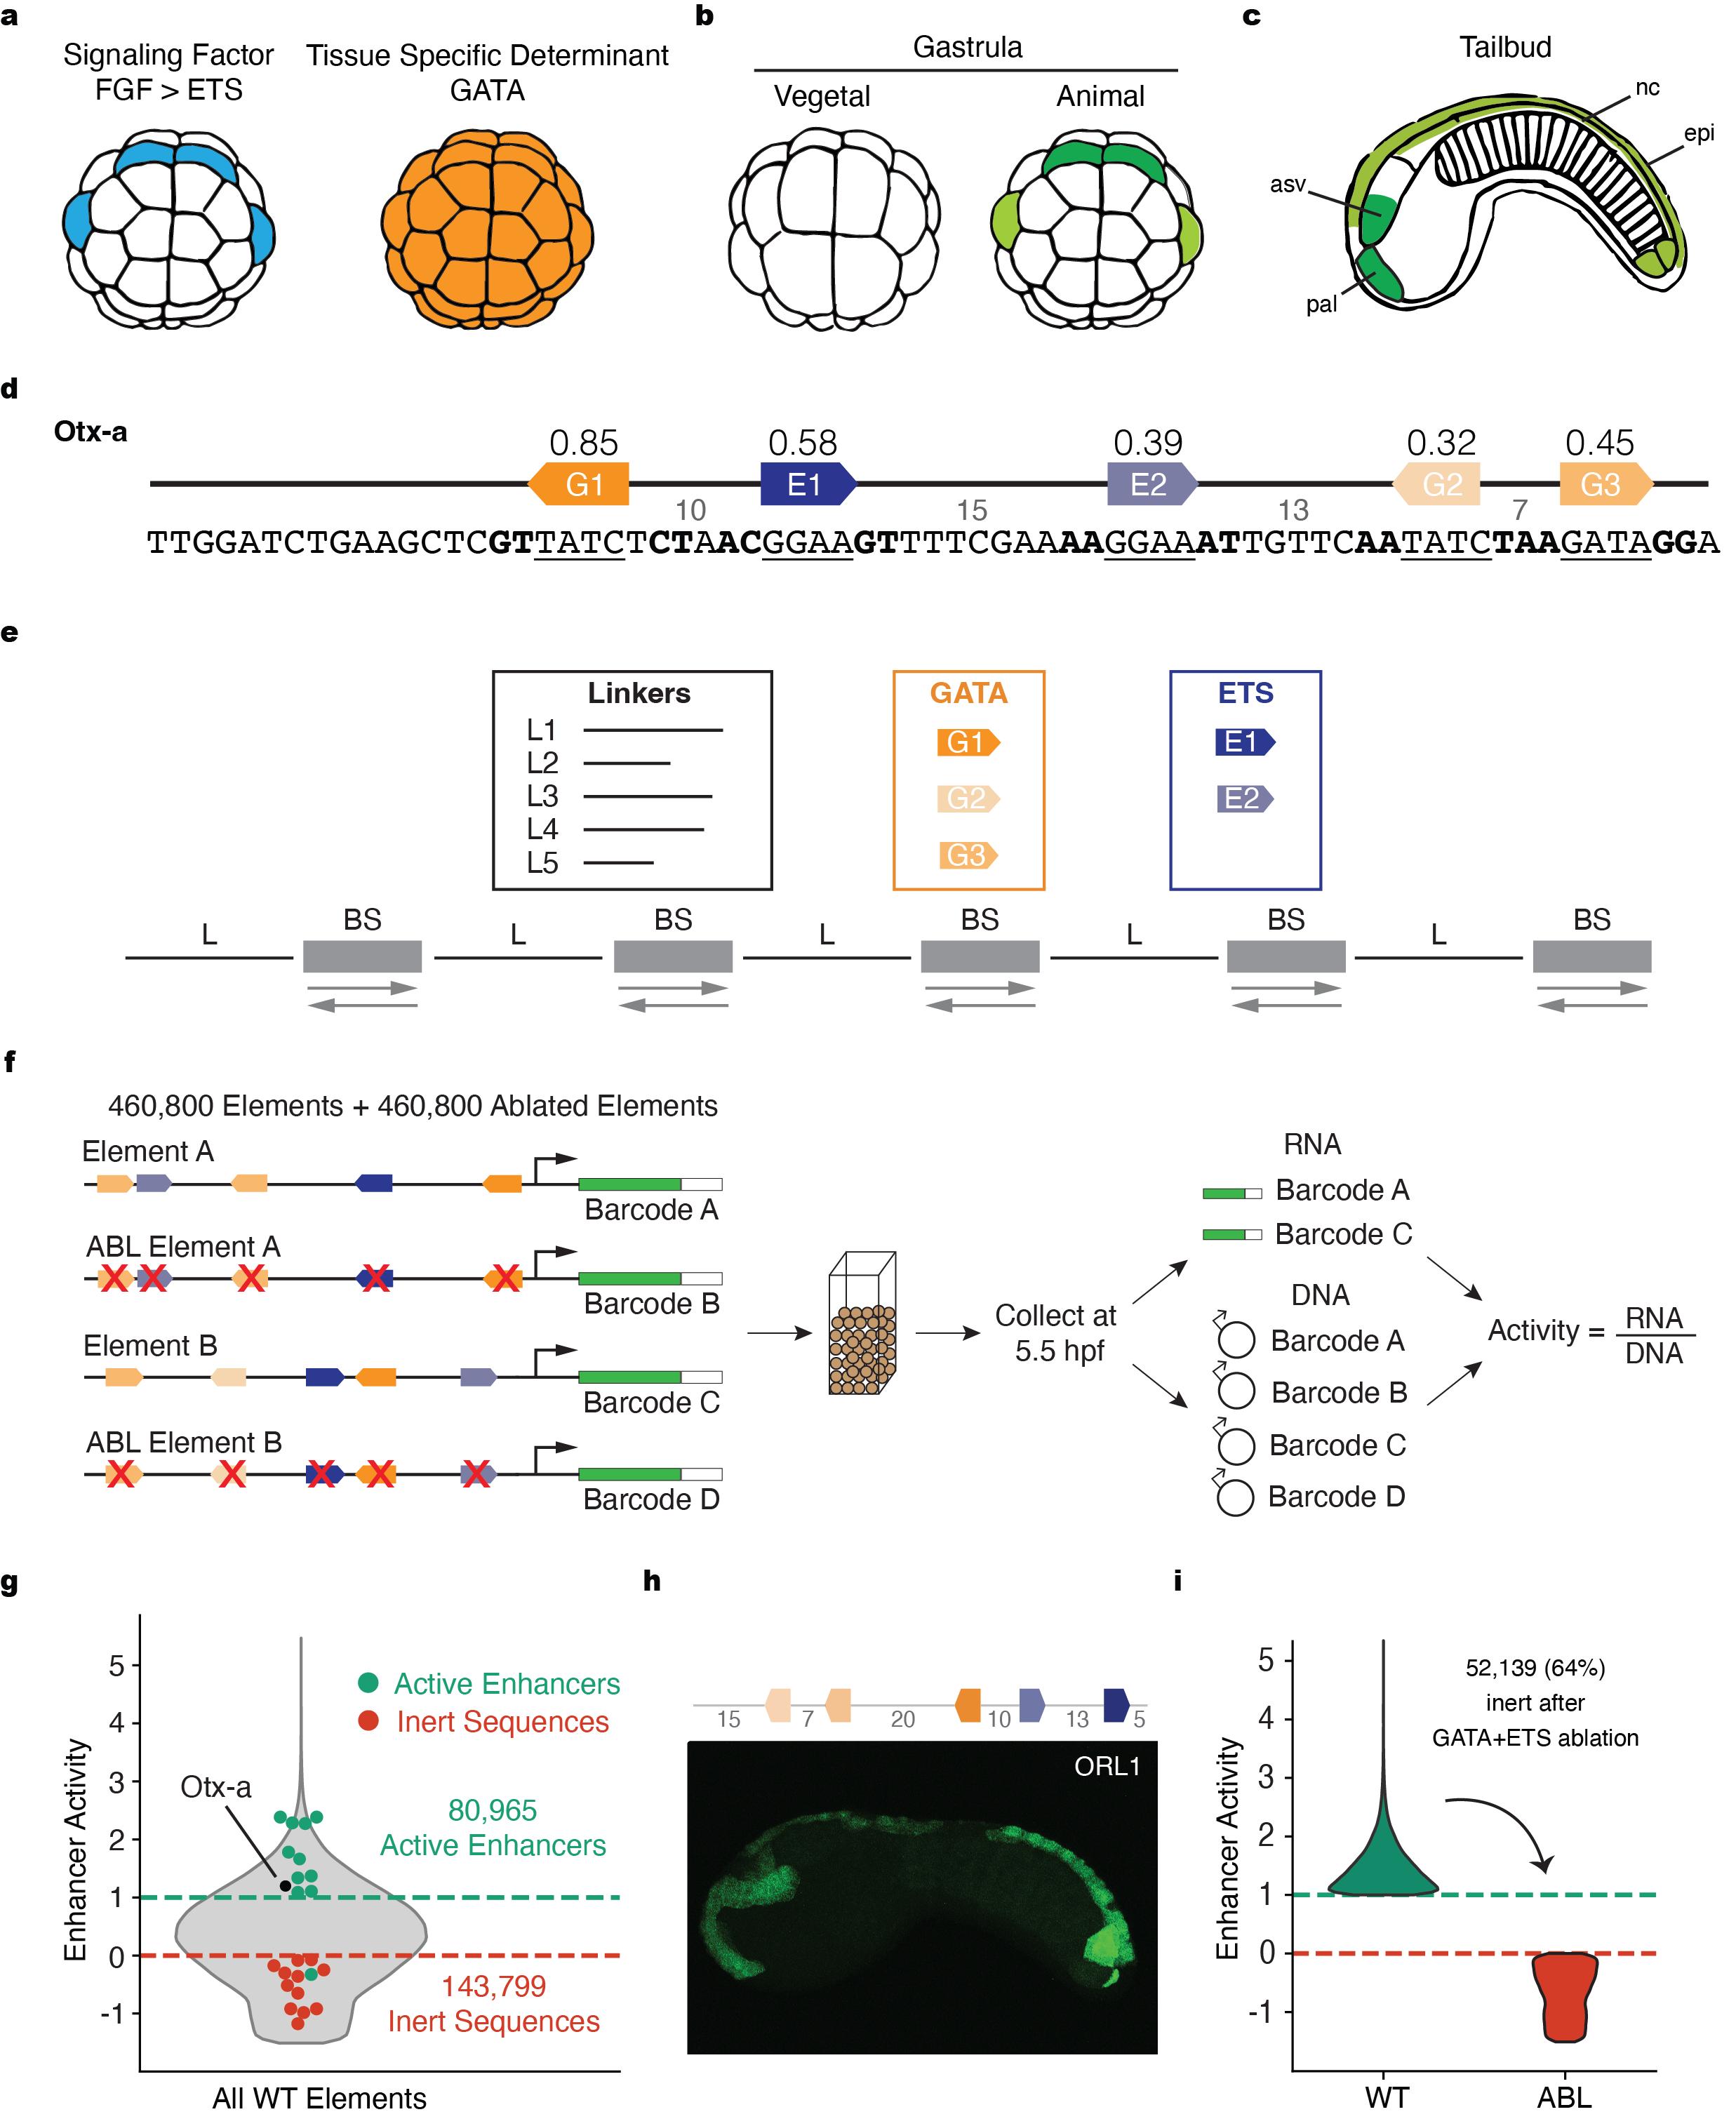
\includegraphics[width=0.9\textwidth, height=0.745\textheight]{2_figures-and-files/Fig1.png}
    \caption[Screening every possible rearrangement of TFBSs in the Otx-a enhancer via MPRA.]{\textbf{Screening every possible rearrangement of TFBSs in the Otx-a enhancer via MPRA.} \textbf{a)} Ciona gastrula embryo at 5.5 hours post fertilization (hpf) showing ectodermal cells in the animal hemisphere. FGF signaling activates ETS in cells (blue). GATA (orange) is expressed in ectodermal cells in the animal hemisphere. FGF signaling also occurs on the vegetal side of the embryo and is not shown. \textbf{b)} The Otx-a enhancer is active in the a6.5 (dark green) and b6.5 (light green) neural lineages in the gastrula stage. \textbf{c)} At the tail-bud stage, expression in the a6.5 lineage gives rise to the palps (pal) and the anterior sensory vesicle (asv), while expression in the b6.5 lineage gives rise to the dorsal epidermis (epi), dorsal nerve cord (nc) and two tail muscle cells (not shown). \textbf{d)} Otx-a contains three GATA and two ETS sites. The GATA and ETS core sequences that hydrogen bond to the TF are underlined, GATA and GGAW respectively. The relative affinity is labelled above each site and is defined by the nucleotides flanking the cores (in bold). Spacing between the sites is shown in gray numbers. \textbf{e)} Otx-a scrambled library (OSL) construction. Each element of the library is created from the five binding sites and five linkers of the Otx-a enhancer, requiring alternation of linker and binding site. Each binding site and linker is used only once per element. Each element therefore has a different order, orientation and spacing of the GATA and ETS sites while maintaining the same sequence content across all elements (Fig. S2). \textbf{f)} Massively parallel reporter assay schematic. Examples of OSL members. Each element and ablated are cloned upstream of a minimal promoter, GFP and a transcribable barcode. All 921,600 elements are electroporated into Ciona fertilized eggs. We extract RNA and DNA barcodes from the mid gastrula-stage embryos (5.5hpf). Enhancer activity score is measured as the ratio of barcode mRNA to barcode DNA (see Methods). \textbf{g)} Enhancer activity distribution of all OSL members. Activity of 23 microscope validated OSL members is shown by colored dots and used to define thresholds for active enhancers (80,965) and inert sequences (143,799) (Fig. S3). \textbf{h)} Tail-bud embryo showing expression of OSL1 in the same neural cells as the WT Otx-a enhancer. \textbf{i)} 52,139 WT elements (64\%) are active enhancers dependent on GATA and ETS sites.}
    \label{fig:2 Figure 1}
\end{figure}

\subsection{TFBS syntax alone accurately predicts enhancer activity}

\begin{figure}[p]
    \centering
    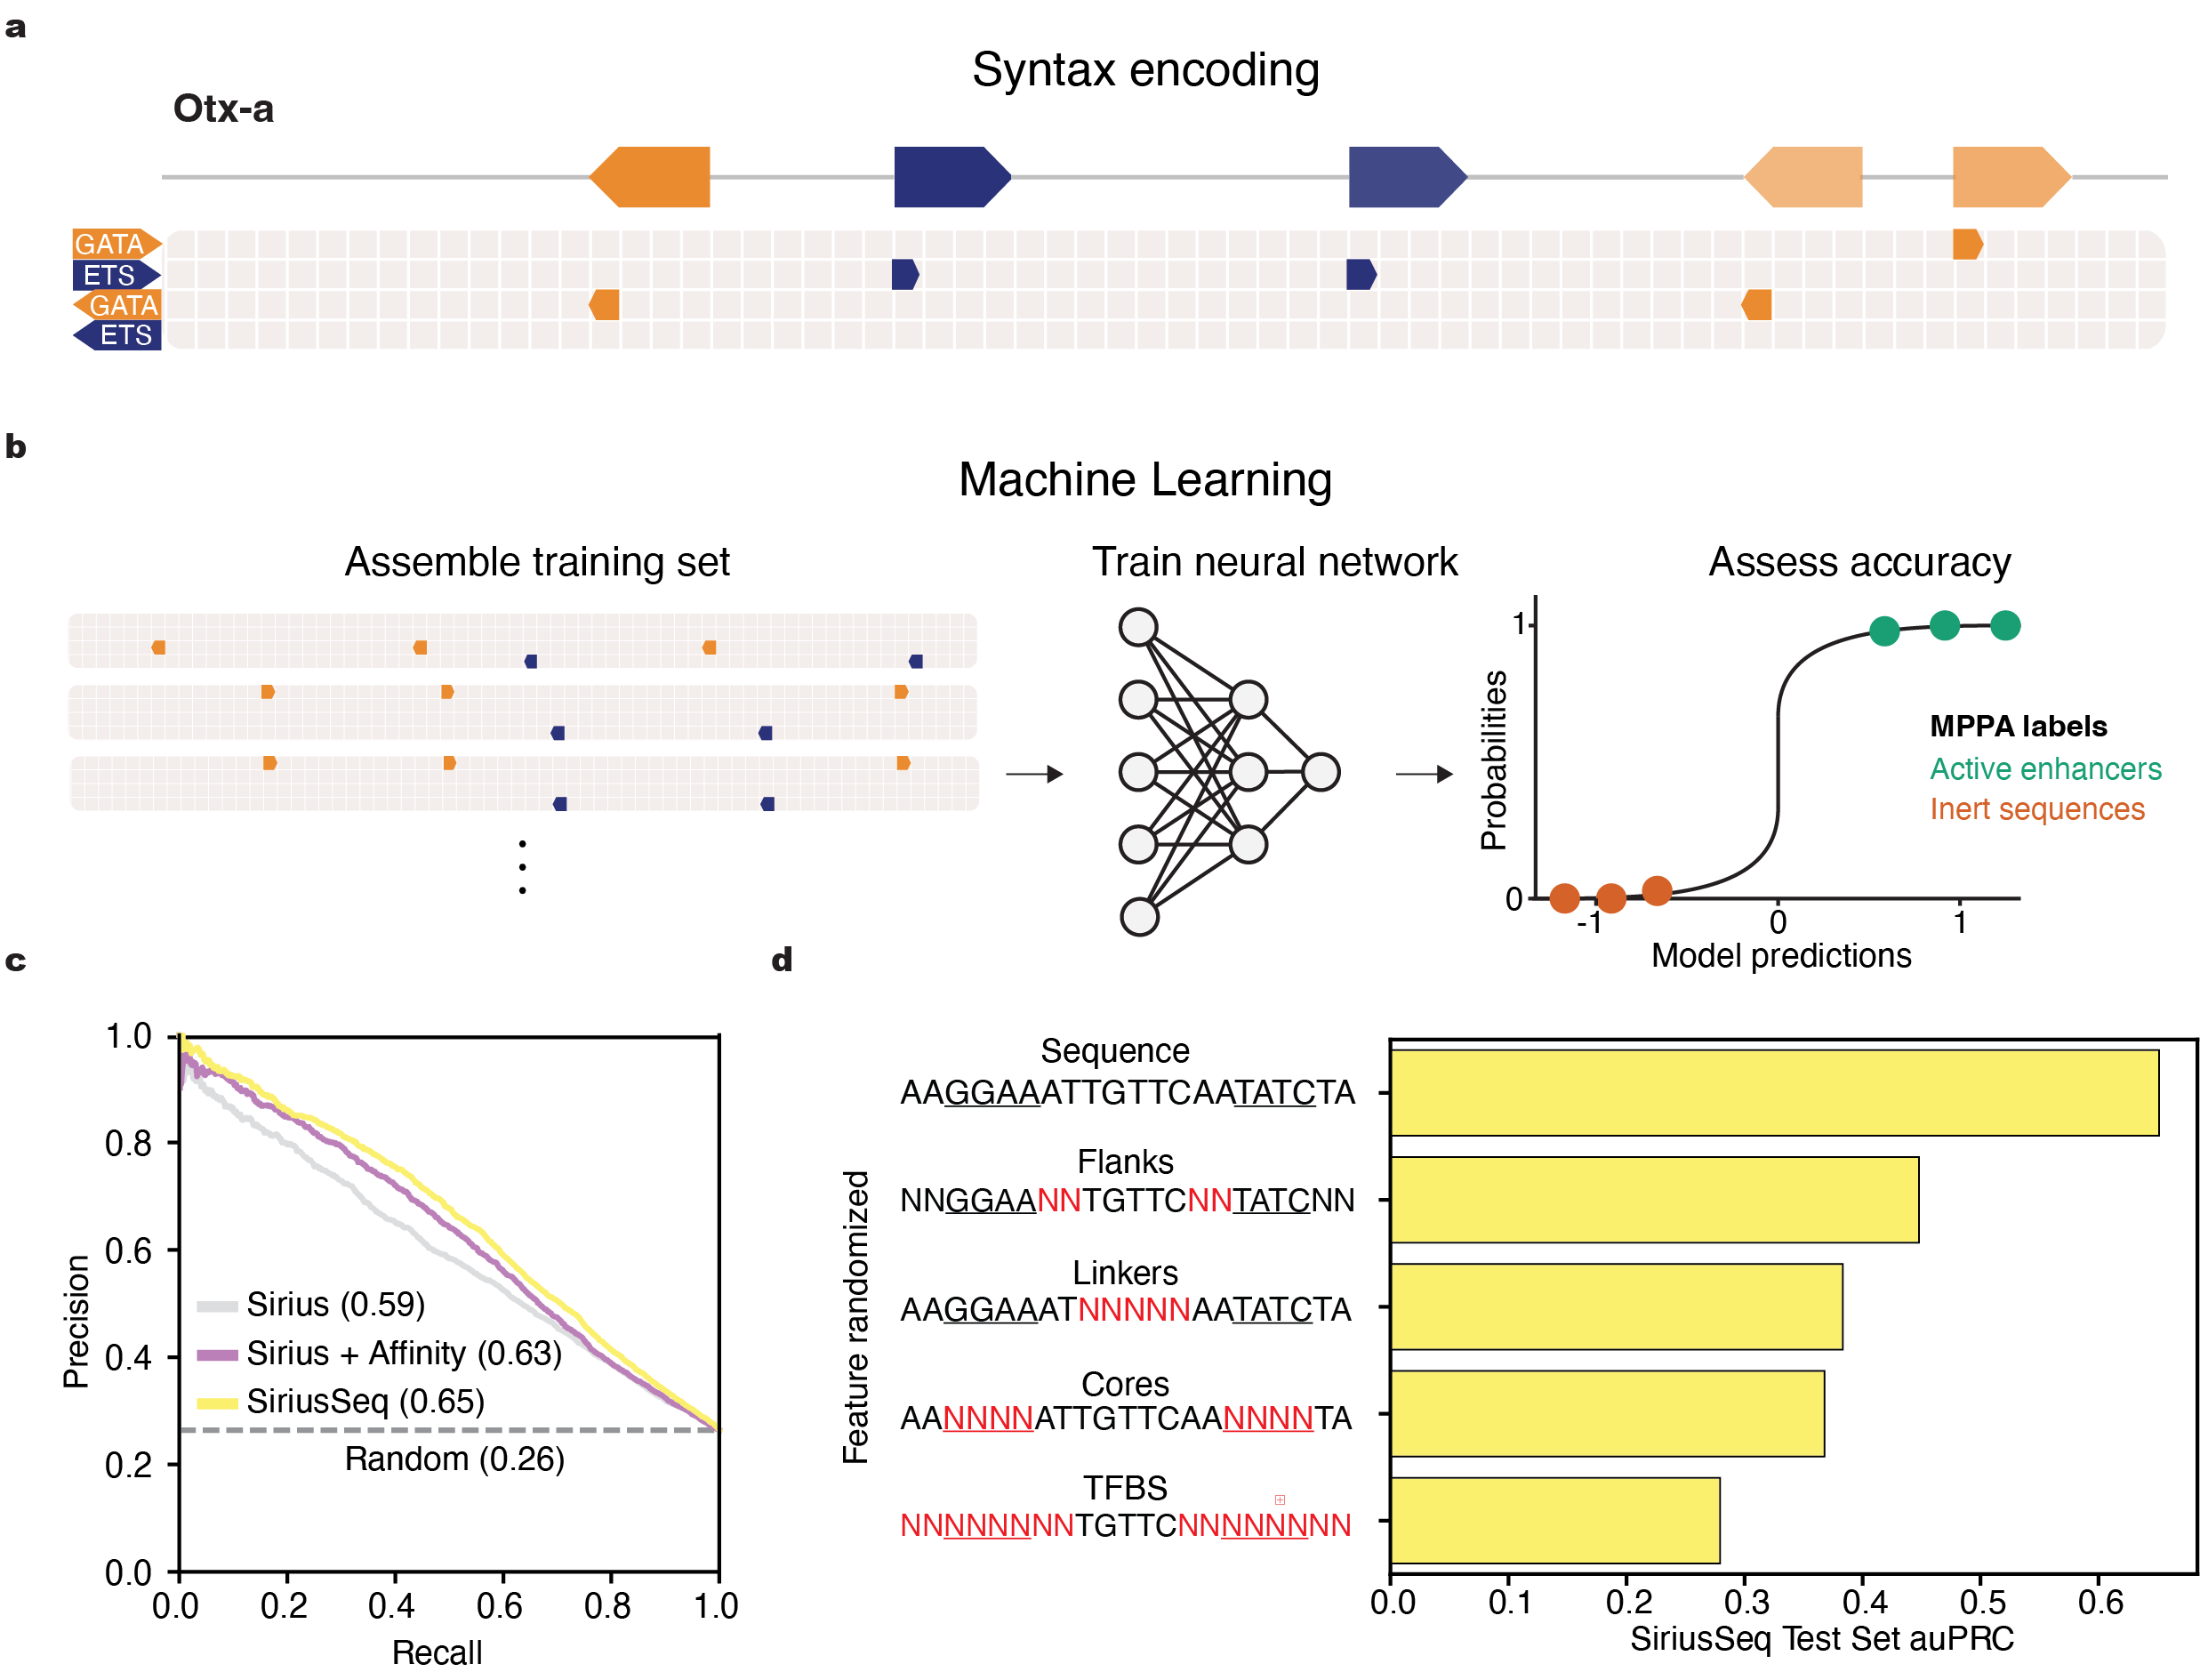
\includegraphics[width=0.9\textwidth, height=0.745\textheight]{2_figures-and-files/Fig2.png}
    \caption[A convolutional neural network trained on TFBS syntax accurately discriminates inert sequences from active enhancers.]{\textbf{A convolutional neural network trained on TFBS syntax accurately discriminates inert sequences from active enhancers.} a) Syntax encoding schematic. Each library member is encoded by the position of GATA and ETS sites in both forward and reverse orientations, capturing order, orientation and spacing of the sites (see Methods). b) Machine learning model training schematic. Library members are partitioned into training, validation and test sets (see Methods). Training sequences are syntax encoded and used to train neural networks. Model predictions are continuous values that are transformed to probabilities via the sigmoid function and compared to MPRA labels to assess classification performance. c) Precision-recall curves for syntax encoding (Sirius), syntax + affinity encoding (Sirius + Affinity) and sequence (SiriusSeq) on held-out test data. Area under the curve (auPRCs) are indicated in parentheses. The dashed grey line indicates the performance of a random classifier. d) SiriusSeq held-out test set auPRCs on sequences with the indicated randomized features.}
    \label{fig:2 Figure 2}
\end{figure}

\subsection{Sirius learns a primarily additive model of TFBS syntax features}

\begin{figure}[p]
    \centering
    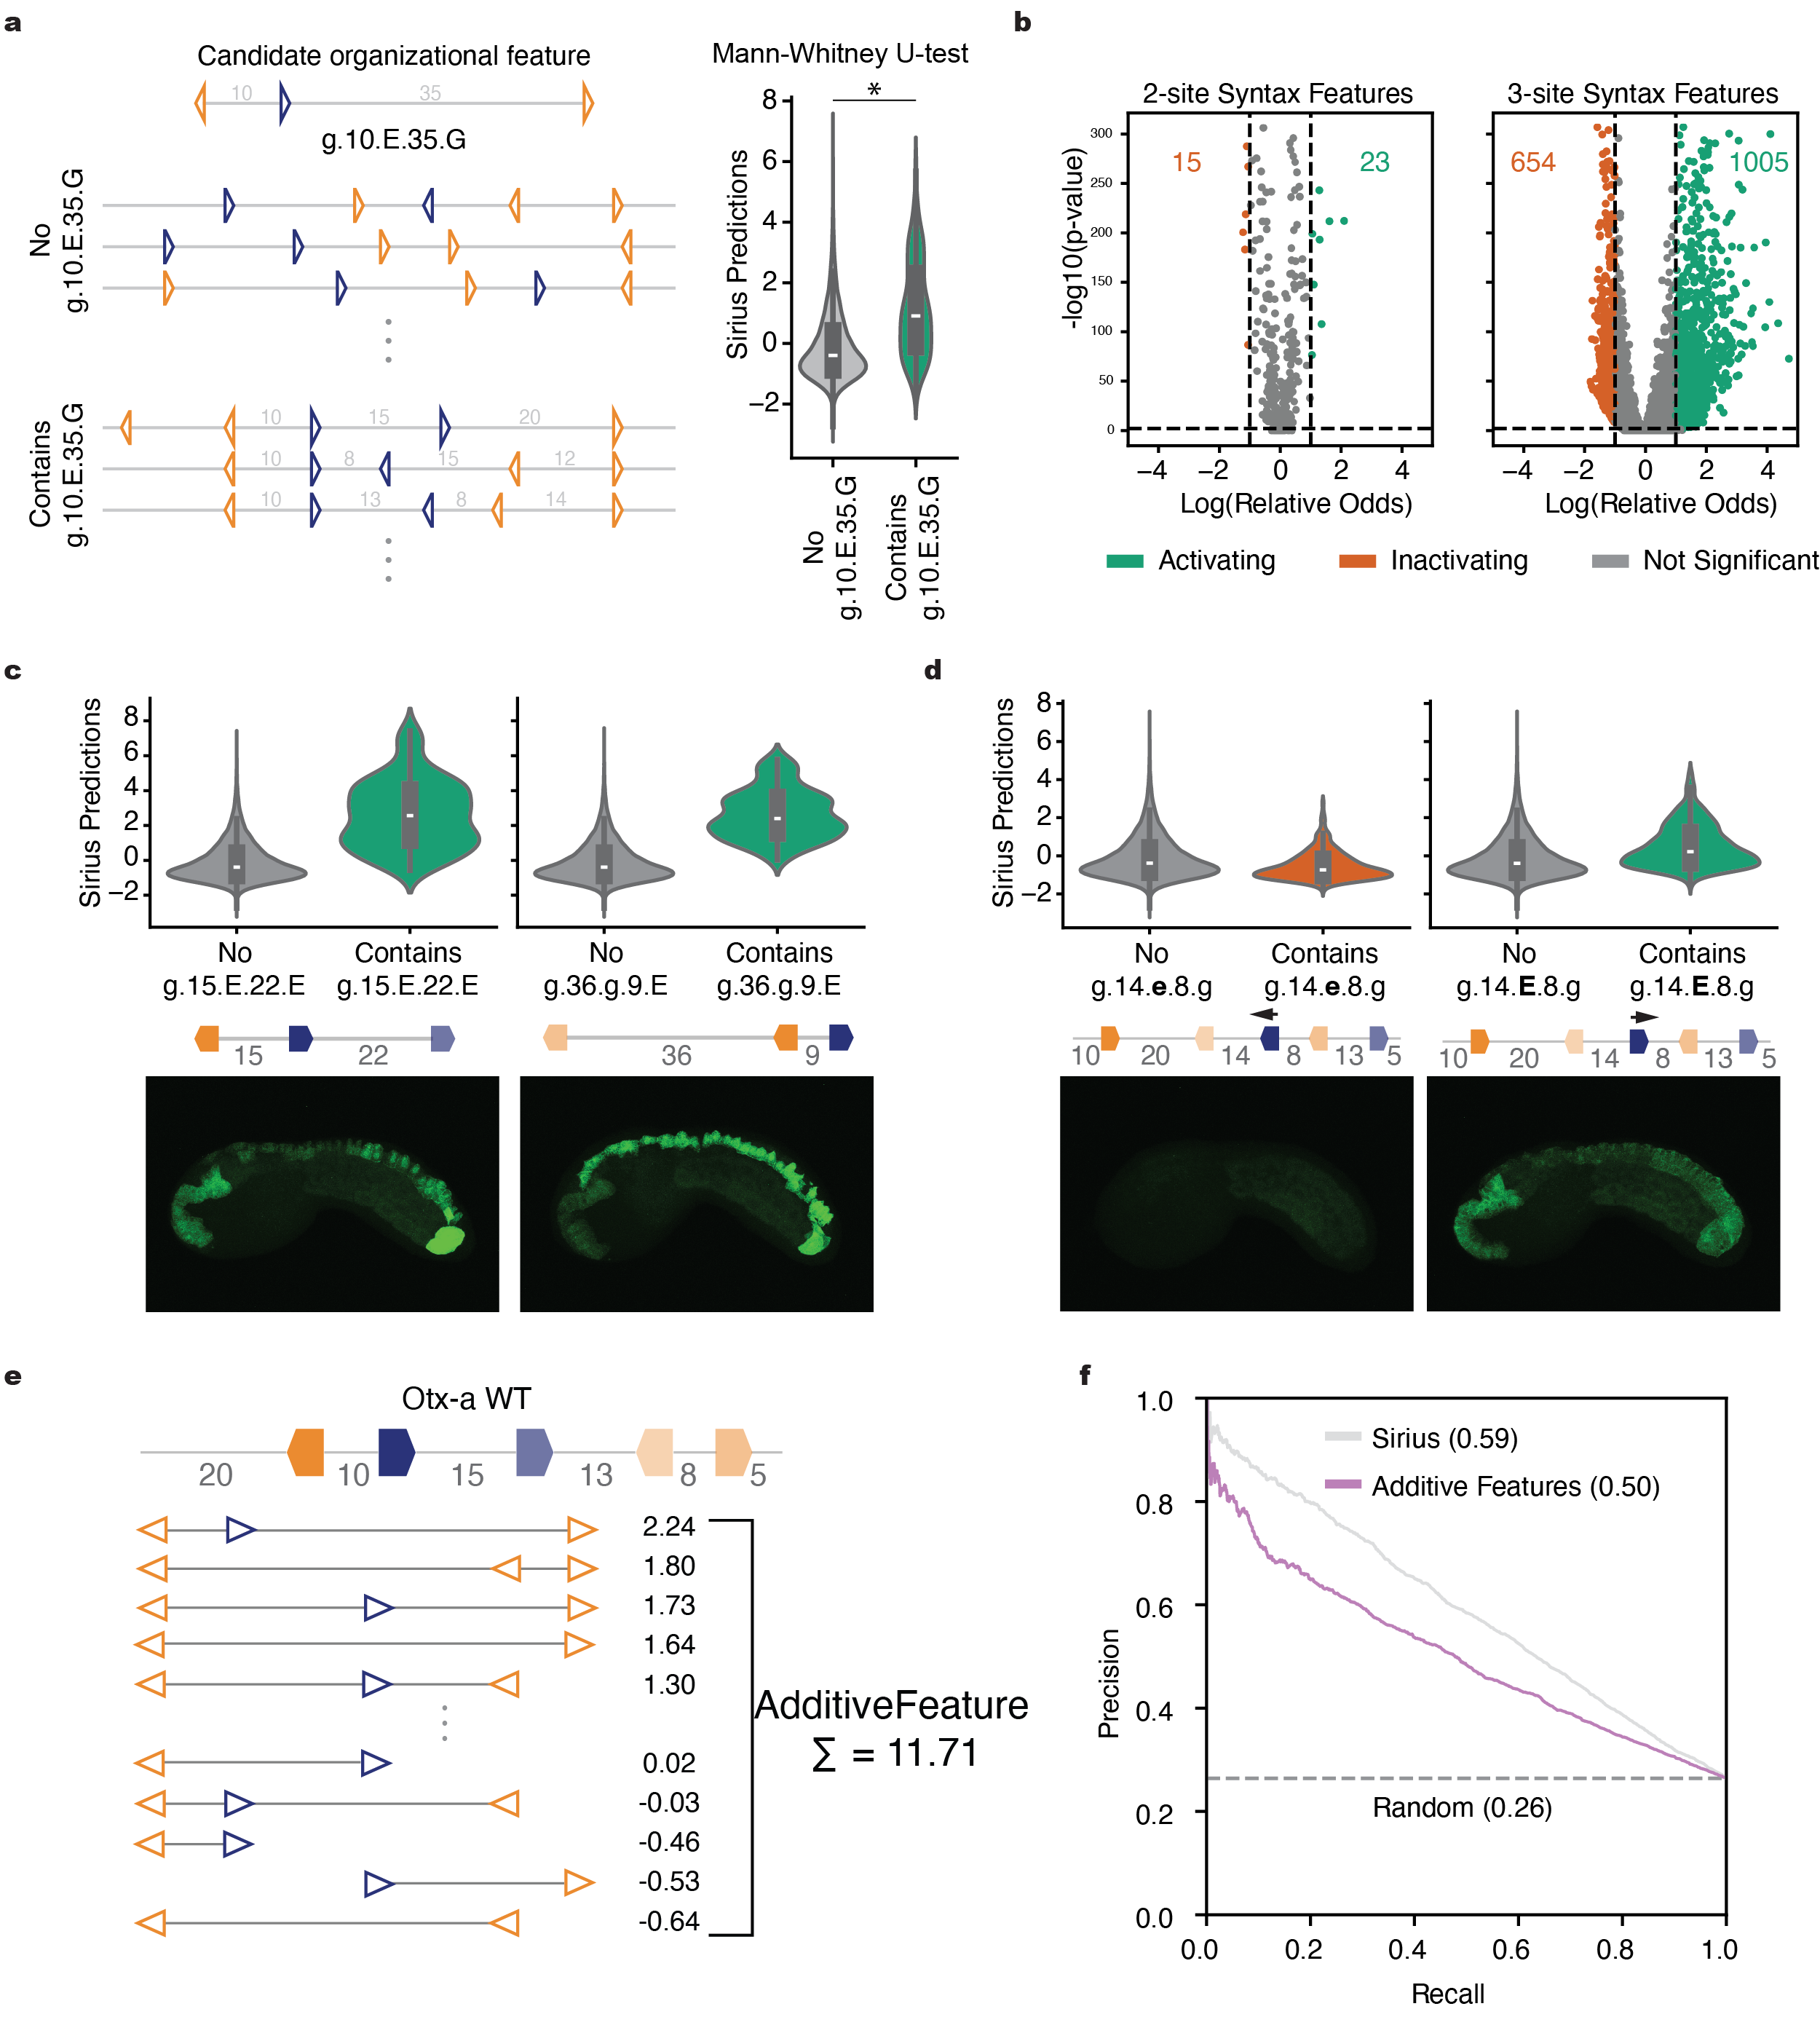
\includegraphics[width=0.9\textwidth, height=0.745\textheight]{2_figures-and-files/Fig3.png}
    \caption[Sirius combines syntax-features in a primarily additive model.]{\textbf{Sirius combines syntax-features in a primarily additive model.} a) Schematic for organizational feature marginalization analysis. Each of 9,022 2-site and 3-site organizational features (see Methods) is tested by splitting up all 460,800 sequences in the library into those that do not contain the feature (No Feature) and those that do (Contains Feature). A Mann-Whitney U-test on the distribution of model predictions for the two groups is used to assign statistical significance (corrected with Benjamini-Hochberg method) and the relative log-odds of mean predictions between groups is used to define an effect size. b) Volcano plots for 2-site (left) and 3-site (right) syntax features where the x-axis shows log2 of the mean relative odds predicted by the model and the y-axis shows -log10(corrected p-value) from the Mann-Whitney U-Test in a). Organizational features are colored based on whether their adjusted p-value is < 0.01 and log2 relative odds is greater than 1 (activating, doubling of odds) or less than -1 (inactivating, halving of odds). c) Two 3-site syntax features that are predicted to be strongly activating act as synthetic active enhancers. d) A single strand flip of an ETS site in a 3-site syntax feature turns it from inactivating (left) to activating (right). e) Schematic for generating a AdditiveFeature score for the Otx-a WT sequence (see Methods). The mean relative odds for each organizational feature contained in the sequence are summed. f) Test set precision-recall curves of AdditiveFeature model compared to full syntax model (Sirius) and random classifier. Numbers in parentheses indicate area under the precision-recall curve (auPRC).}
    \label{fig:2 Figure 3}
\end{figure}

\subsection{Sirius enables accurate tissue-specific enhancer design}

\begin{figure}[p]
    \centering
    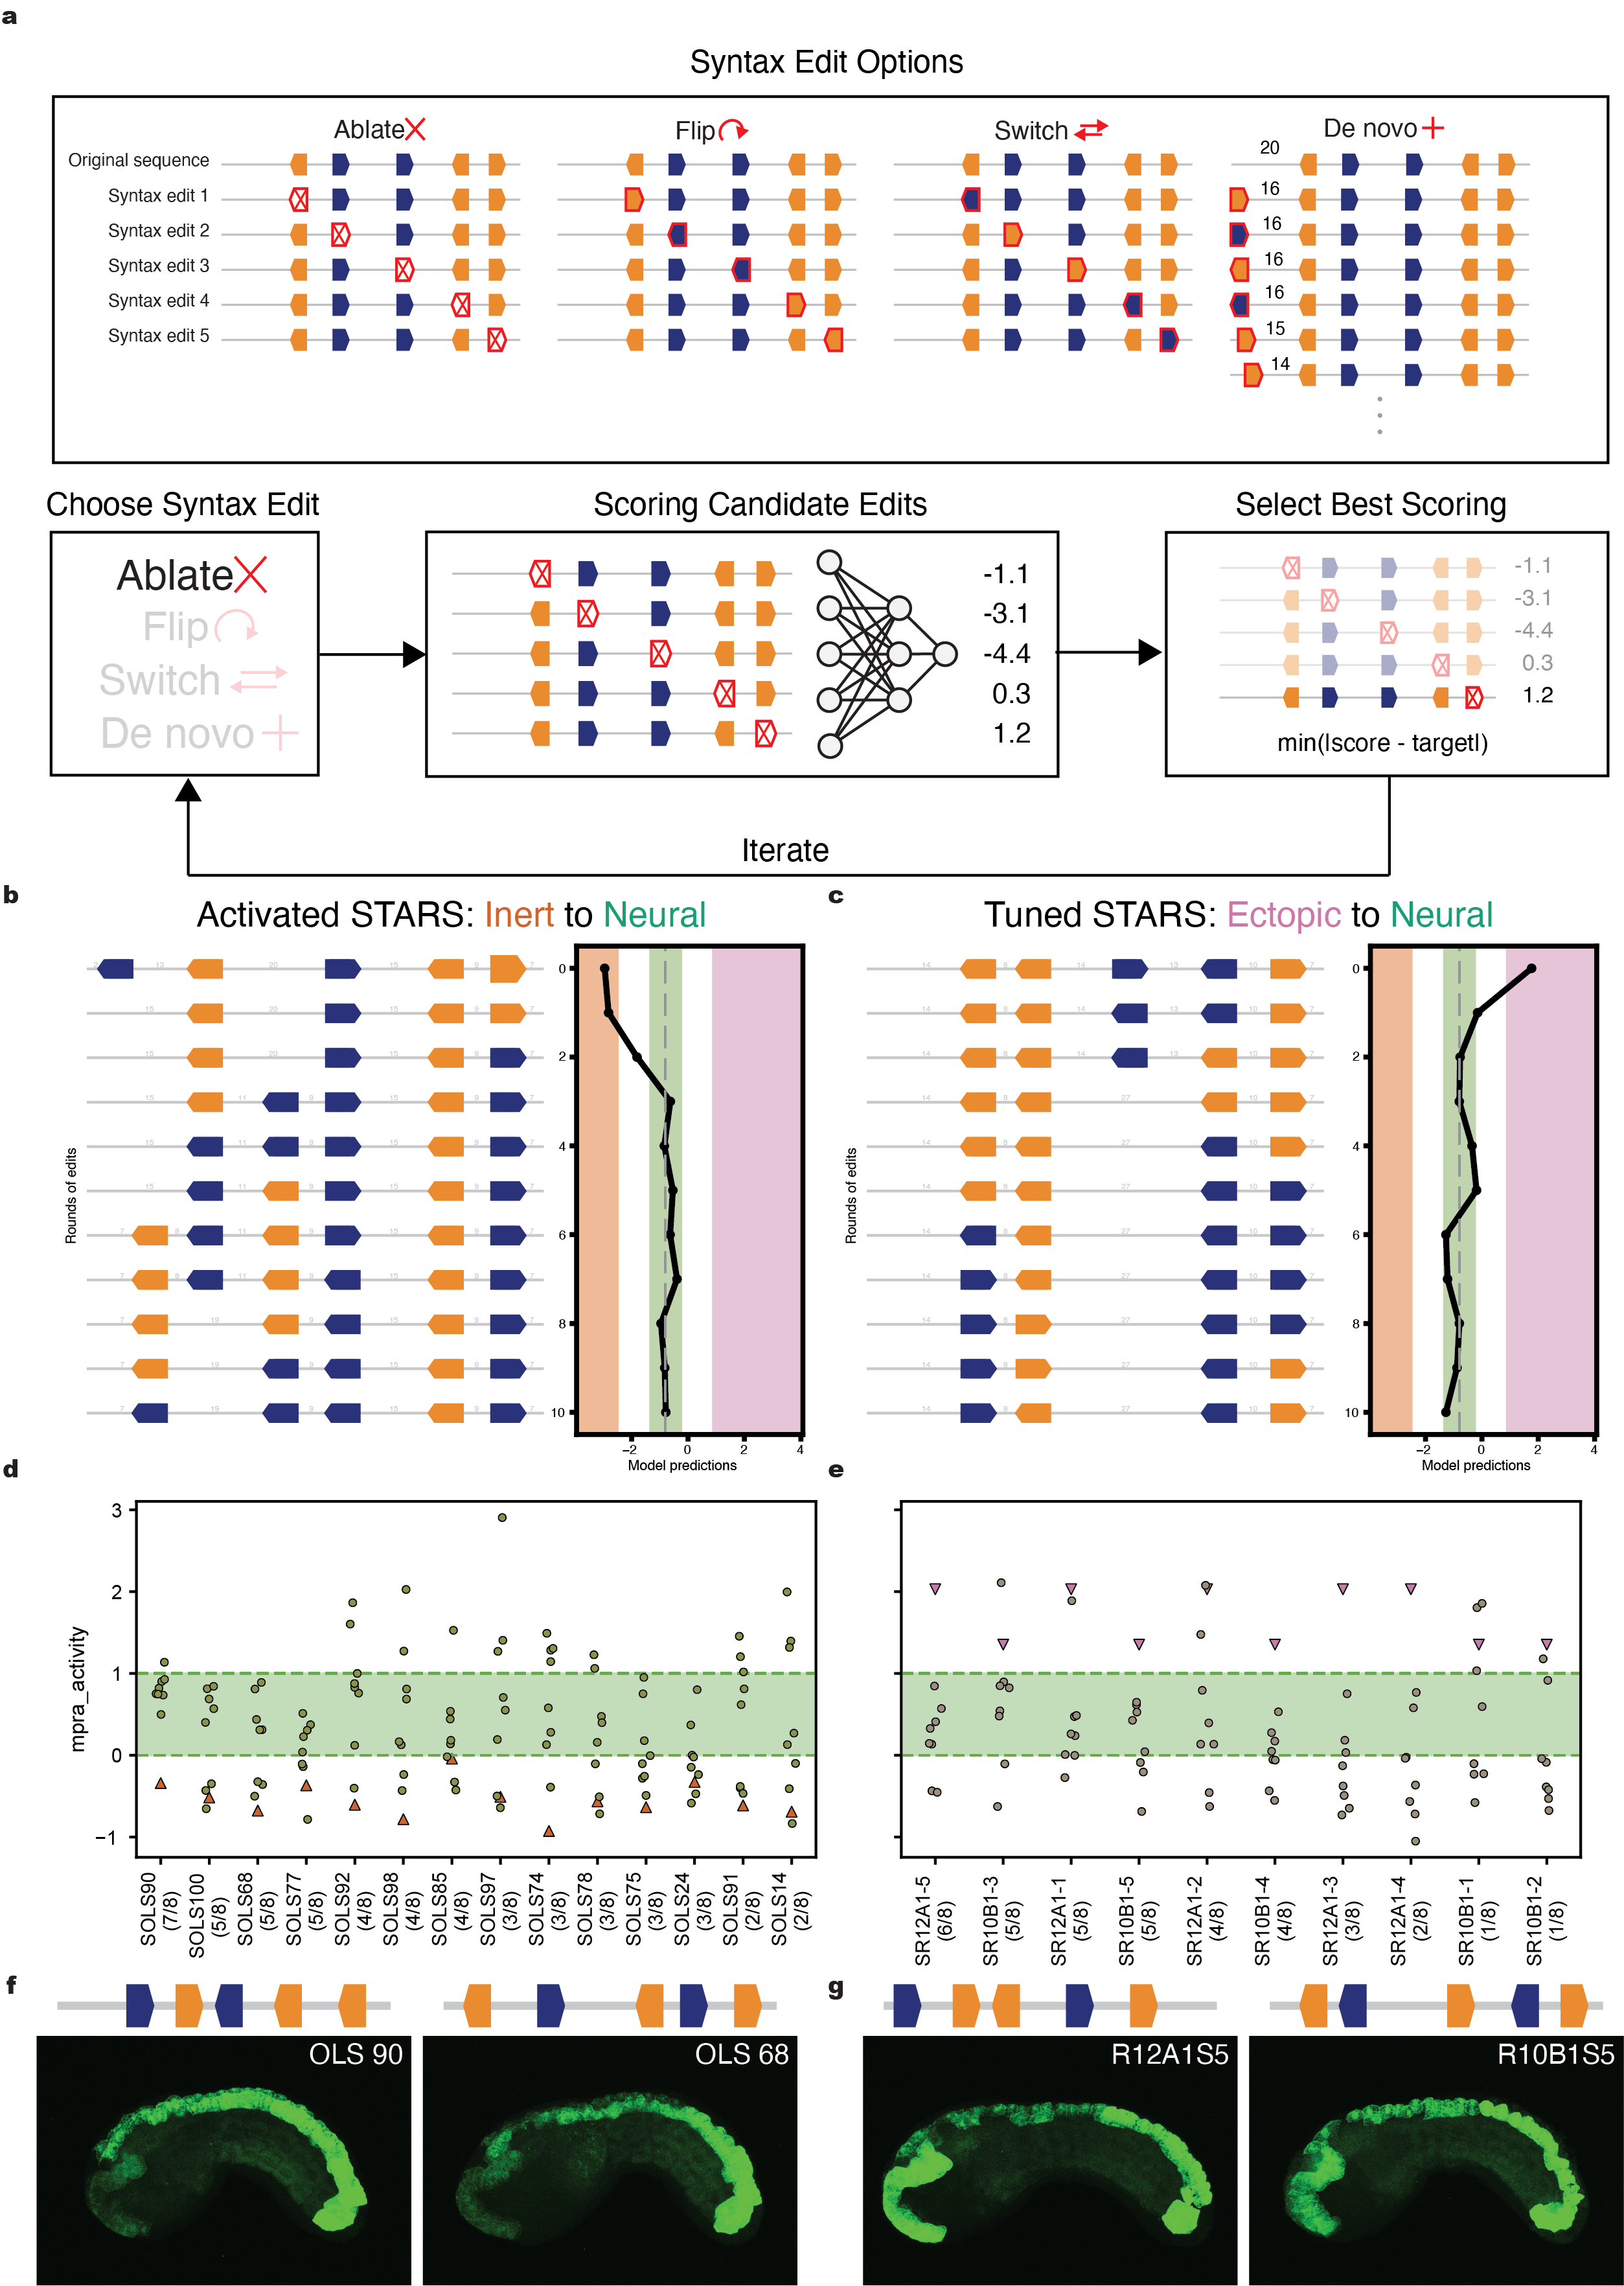
\includegraphics[width=0.9\textwidth, height=0.745\textheight]{2_figures-and-files/Fig4.png}
    \caption[Syntax-driven design of tissue-specific enhancers.]{\textbf{Syntax-driven design of tissue-specific enhancers.} a) Schematic of design process. We define four types of syntax edit that each generate a set of candidate syntaxes to score with the model. In each round of design, a syntax edit type is selected at random and candidate syntaxes are generated. Activity is then predicted with Sirius and transformed to a score using a chosen objective function. The highest scoring syntax is then selected for the next round of editing. Examples of activated (b) and tuned (c) STARS. Left, binding site syntaxes of sequences at each round. Right, model prediction for each round. Background colors are determined by the interquartile ranges of the Inert Sequence, Neural Enhancer and Ectopic Enhancer distributions shown in Fig. S10c. STARS MPRA analysis for activated e) and tuned f) STARS. Y-axis shows change in measured activity of the designed sequence with respect to the measured activity of its starting sequence. Each syntax was used to generate eight different DNA sequences with differing flanks and linkers. Each point (sequence) is colored by the classification label assigned using thresholds from internal controls validated with fluorescence microscopy (Fig. S13.b,c). Barplot on top indicates the number of GATA and ETS sites in the respective designed syntax.}
    \label{fig:2 Figure 4}
\end{figure}

\subsection{Features beyond GATA/ETS syntax improve prediction of genomic enhancer function}

\begin{figure}[p]
    \centering
    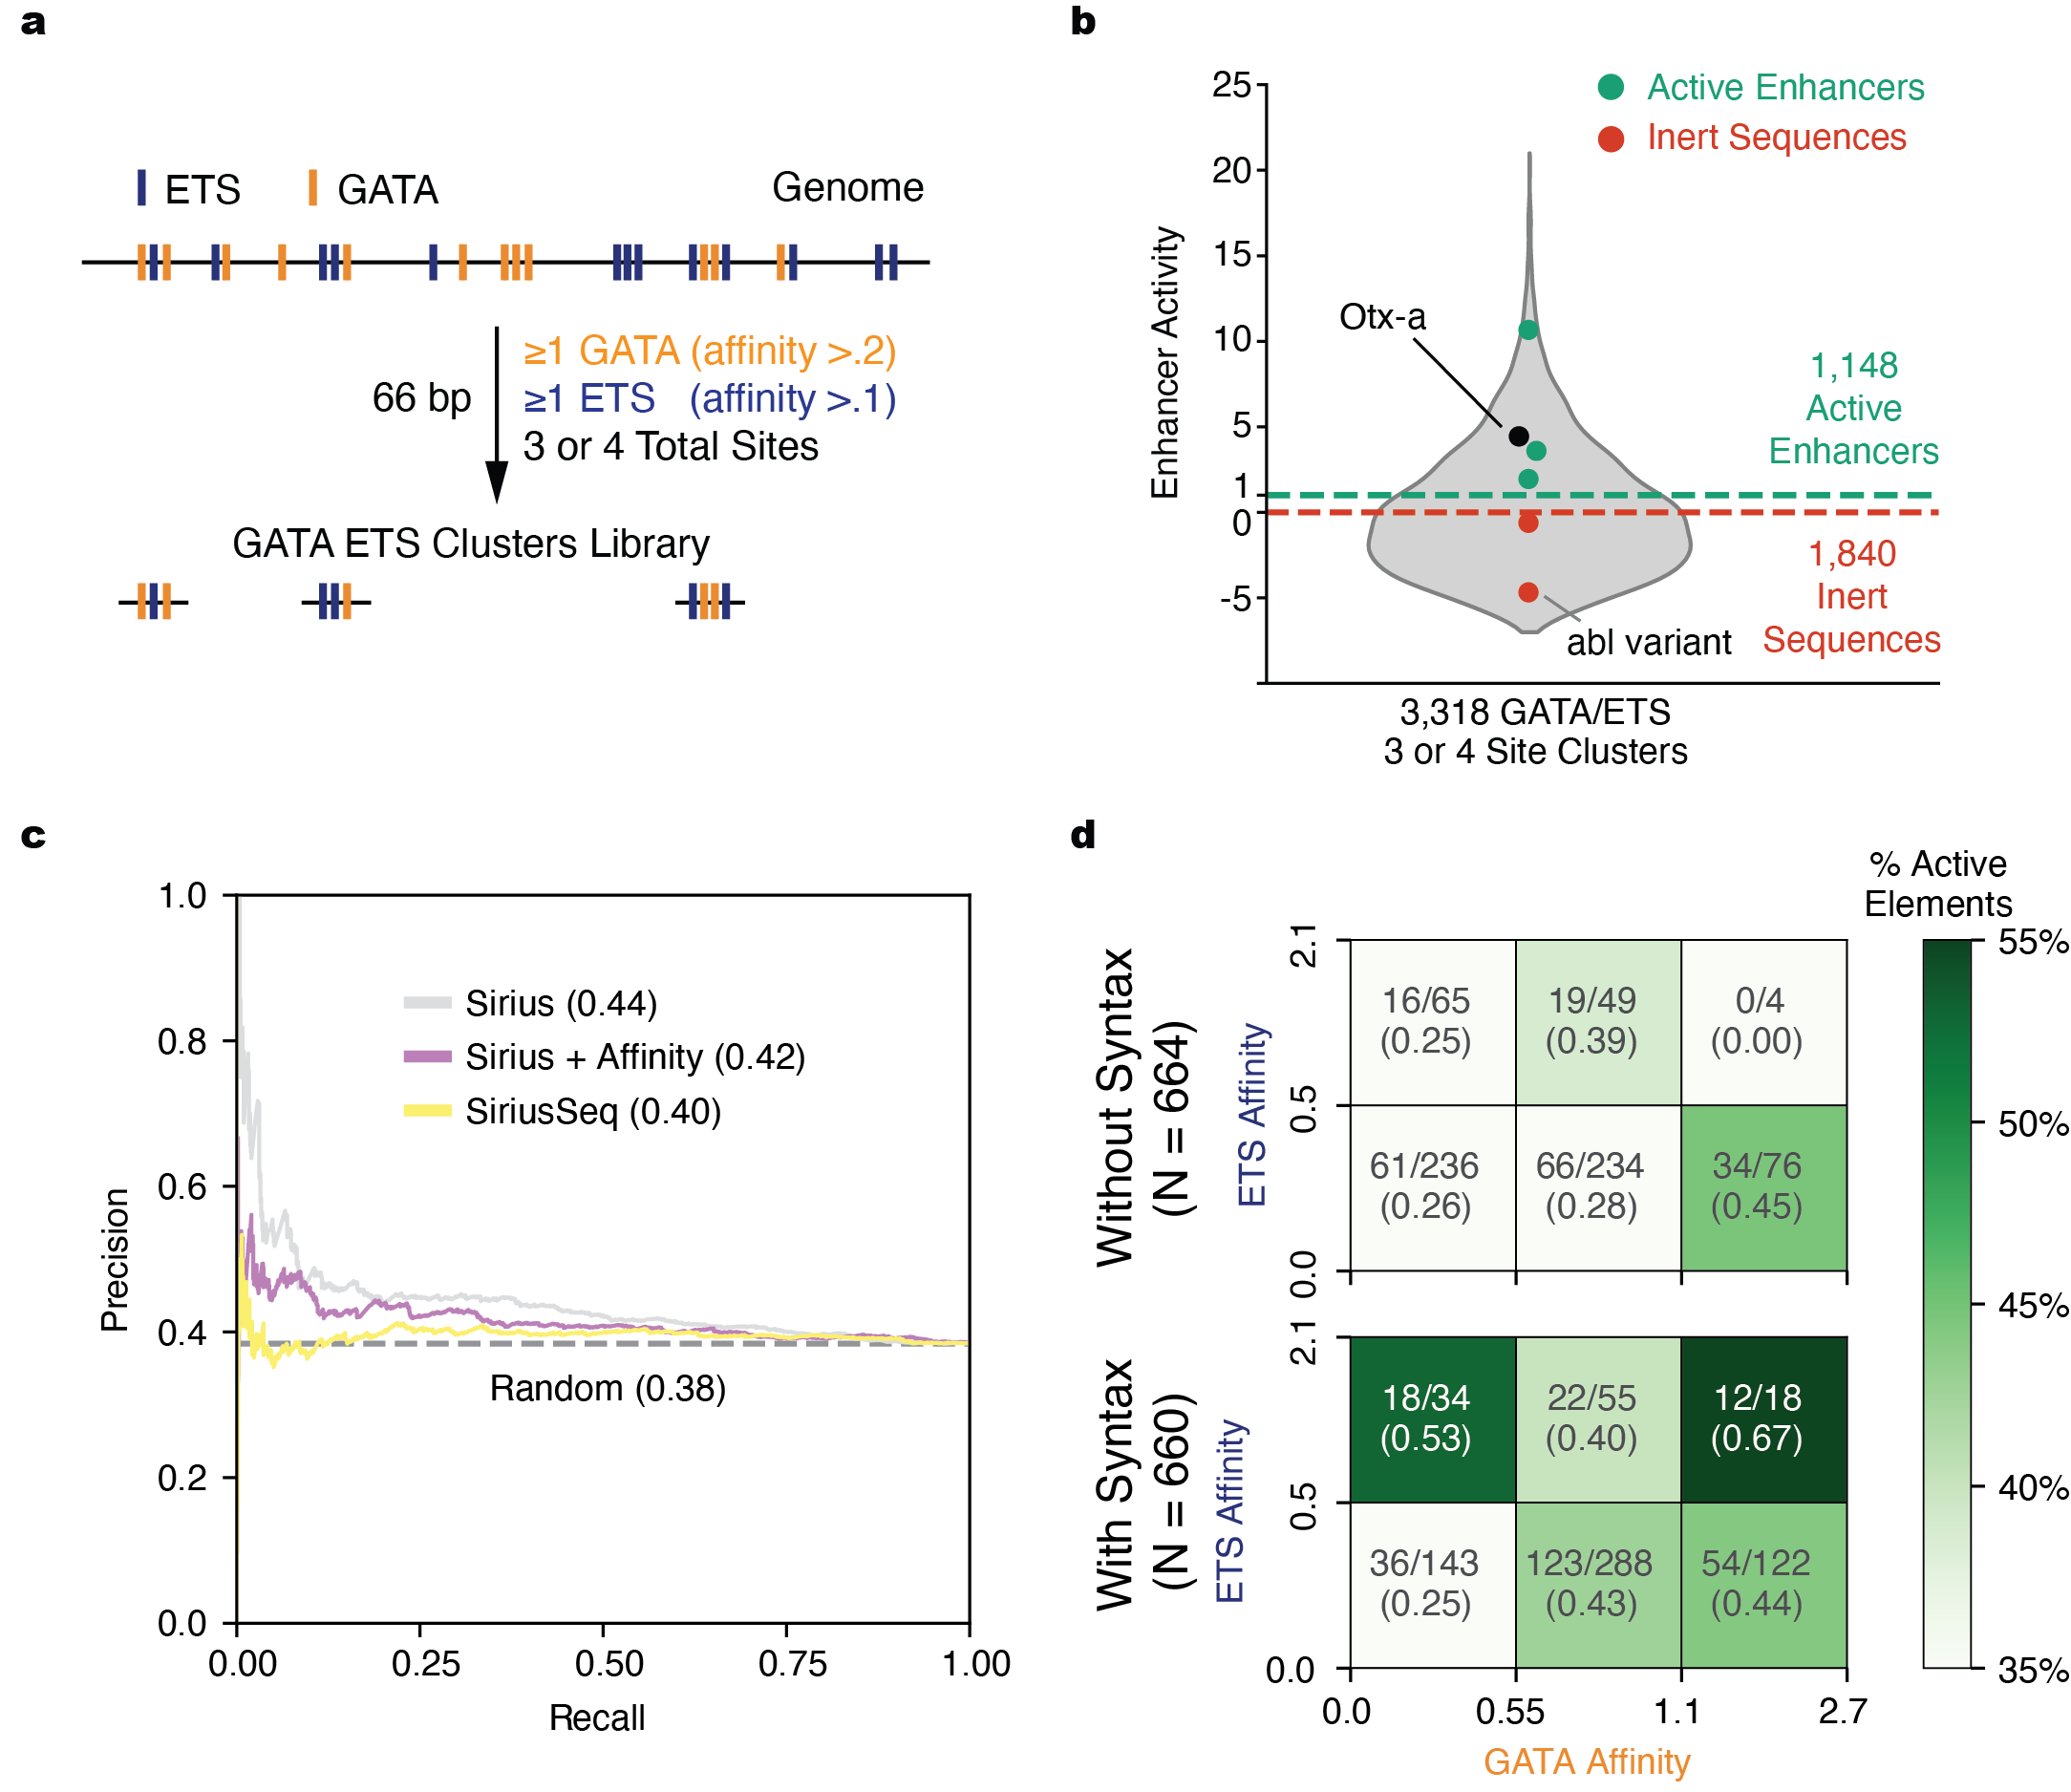
\includegraphics[width=0.9\textwidth, height=0.745\textheight]{2_figures-and-files/Fig5.png}
    \caption[OSL models predict activity of genomic clusters of ETS and GATA sites.]{\textbf{OSL models predict activity of genomic clusters of ETS and GATA sites.} a) Schematic showing search for clusters of ETS and GATA binding sites. Each element contains at least one GATA site (relative affinity > 0.2) and one ETS site (relative affinity > 0.1). b) Enhancer activity of the 3,318 genomic elements tested in Ciona embryos. 1,148 elements are active enhancers while 1,840 elements are inert sequences. Activity of six internal controls are shown as the colored points: Otx-a (black), three positive controls (green), and two negative controls (red). c) Precision-recall curves for OSL trained models on genomic clusters: Syntax encoding (Sirius), syntax + affinity encoding (Sirius + Affinity) and sequence (SiriusSeq). Areas under the curve (auPRCs) are indicated in parentheses. The dashed grey line indicates the performance of a random classifier. d) Percent of active enhancers within each group separated based on affinity and syntax. Each element is placed in a bin based on the summed affinity of ETS (heatmap Y-axis), summed affinity of GATA (heatmap X-axis) and the syntax group. Top heatmap contains elements with in the bottom 20th percentile of Sirius scores. Lower heatmap contains the elements in the top 20th percentile of Sirius scores.}
    \label{fig:2 Figure 5}
\end{figure}

%%%%%%%%%%%%%%%%%%%%%%%%%%%%%%%%%%%%%%%%%%%%%%%%%%%%%%%%%%%%%%%%%%%%%%%%%%%%%%%%
\section{Discussion}
%%%%%%%%%%%%%%%%%%%%%%%%%%%%%%%%%%%%%%%%%%%%%%%%%%%%%%%%%%%%%%%%%%%%%%%%%%%%%%%%

%%%%%%%%%%%%%%%%%%%%%%%%%%%%%%%%%%%%%%%%%%%%%%%%%%%%%%%%%%%%%%%%%%%%%%%%%%%%%%%%
\section{Materials and Methods}
%%%%%%%%%%%%%%%%%%%%%%%%%%%%%%%%%%%%%%%%%%%%%%%%%%%%%%%%%%%%%%%%%%%%%%%%%%%%%%%%

\subsection{Ciona}

\section{Data availability}

\section{Code availability}

\section{Data availability}
